% !TEX program = xelatex
\documentclass[a4paper]{article}
\usepackage[UTF8]{ctex}
\setCJKmainfont{SimSun}[BoldFont=SimHei,ItalicFont=KaiTi]
\setCJKsansfont{SimHei}
\usepackage[top=3mm,bottom=3mm,left=3mm,right=3mm]{geometry}
\usepackage{amsmath,amssymb,bm}
\usepackage{multicol}
\usepackage{tikz}
\usetikzlibrary{arrows.meta,calc}
\usepackage[dvipsnames]{xcolor}
\usepackage{array,tabularx}
\pagestyle{empty}
\setlength{\parindent}{0pt}
\setlength{\parskip}{0pt}
\setlength{\columnsep}{2.0mm}
\setlength{\columnseprule}{0.12pt}
\setlength{\tabcolsep}{1.0pt}
\setlength{\fboxsep}{0.65pt}
\renewcommand{\baselinestretch}{0.66}
\definecolor{h}{HTML}{0B3D91}
\definecolor{b}{HTML}{1565C0}
\definecolor{r}{HTML}{B71C1C}
\definecolor{o}{HTML}{E65100}
\definecolor{g}{HTML}{1B5E20}
\definecolor{bg}{HTML}{EEF3FF}
\definecolor{warnbg}{HTML}{FFF2E6}
\definecolor{grid}{HTML}{D6DEE8}
\newsavebox{\fitbox}
\newcommand{\fitmath}[2][\dimexpr\linewidth-4pt\relax]{\sbox{\fitbox}{$\displaystyle #2$}\ifdim\wd\fitbox>#1\resizebox{#1}{!}{$\displaystyle #2$}\else\usebox{\fitbox}\fi}
\newcommand{\E}[1]{\colorbox{bg}{\fitmath{#1}}}
\newcommand{\Hh}[1]{\vspace{0.35pt}{\fontsize{6.1}{6.25}\selectfont\bfseries\color{white}\colorbox{h}{\strut\ #1\ }}\par\vspace{0.2pt}}
\newcommand{\linea}[2]{\textbf{\color{b}#1}：#2\par}
\newcommand{\warn}[1]{\colorbox{warnbg}{\begin{minipage}{\dimexpr\linewidth-2\fboxsep\relax}\fontsize{4.72}{4.95}\selectfont\textbf{\color{r}错}：#1\end{minipage}}\par}
\newcommand{\modu}[5]{\vspace{0.35pt}\noindent\fcolorbox{grid}{white}{\begin{minipage}{0.976\linewidth}\fontsize{4.72}{4.95}\selectfont\textbf{\color{h}#1}\par\linea{题干}{#2}\linea{第一行}{#3}\linea{公式链}{#4}\linea{扩展/简答/错}{#5}\end{minipage}}\par}
\newcommand{\mini}[2]{\vspace{0.25pt}\noindent\fcolorbox{grid}{white}{\begin{minipage}{0.976\linewidth}\fontsize{4.72}{4.95}\selectfont\textbf{\color{h}#1}\par #2\end{minipage}}\par}
\newcommand{\formula}[2]{\mini{#1}{\colorbox{bg}{\begin{minipage}{\dimexpr\linewidth-2\fboxsep\relax}\centering\fontsize{4.55}{4.75}\selectfont #2\end{minipage}}}}
\newcommand{\pipeicon}{\begin{center}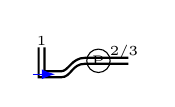
\begin{tikzpicture}[>=Latex,scale=.38,every node/.style={font=\tiny}]
\draw[thick](0,1)--(0,0)--(.75,0)..controls(1.1,0)and(1.1,.45)..(1.55,.45)--(3.0,.45);
\draw[thick](.2,1)--(.2,.2)--(.75,.2)..controls(1.0,.2)and(1.1,.65)..(1.55,.65)--(3.0,.65);
\draw[->,blue](-.2,.1)--(.55,.1);\node[circle,draw,inner sep=1pt] at (2.0,.55){P};\node at(.1,1.2){1};\node at(2.85,.85){2/3};
\end{tikzpicture}\end{center}}
\newcommand{\lavalicon}{\begin{center}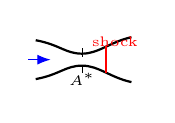
\begin{tikzpicture}[>=Latex,scale=.38,every node/.style={font=\tiny}]
\draw[thick](0,.65)..controls(.8,.5)and(1.0,.2)..(1.55,.2)..controls(2.1,.2)and(2.5,.6)..(3.2,.75);
\draw[thick](0,-.65)..controls(.8,-.5)and(1.0,-.2)..(1.55,-.2)..controls(2.1,-.2)and(2.5,-.6)..(3.2,-.75);
\draw[dashed](1.55,-.45)--(1.55,.45);\node at(1.55,-.65){$A^*$};\draw[->,blue](-.25,0)--(.5,0);\draw[red,thick](2.35,-.45)--(2.35,.45);\node[red]at(2.65,.6){shock};
\end{tikzpicture}\end{center}}
\newcommand{\cvicon}{\begin{center}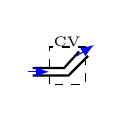
\begin{tikzpicture}[>=Latex,scale=.38,every node/.style={font=\tiny}]
\draw[thick](0,.3)--(1.2,.3)--(1.85,.95);\draw[thick](0,.55)--(1.05,.55)--(1.55,1.1);\draw[dashed](.55,.0)rectangle(1.75,1.25);
\draw[->,blue](-.15,.42)--(.55,.42);\draw[->,blue](1.47,.95)--(2.05,1.32);\node at(1.15,1.43){CV};
\end{tikzpicture}\end{center}}
\newcommand{\poticon}{\begin{center}\begin{tikzpicture}[>=Latex,scale=.36,every node/.style={font=\tiny}]
\foreach \y in{-.35,0,.35}{\draw[->,blue](-.1,\y)--(.8,\y);}\draw[thick](1.15,0)circle(.32);\node at(1.15,-.55){圆柱};
\draw[fill=black](2.1,0)circle(.04);\node[above]at(2.1,0){源};\draw[thick](2.75,-.5)..controls(3.2,-.75)and(3.6,-.75)..(4.0,-.5);
\end{tikzpicture}\end{center}}
\newcommand{\stressicon}{\begin{center}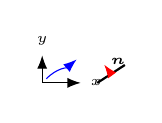
\begin{tikzpicture}[>=Latex,scale=.35,every node/.style={font=\tiny}]
\draw[->](0,0)--(1.4,0)node[right]{$x$};\draw[->](0,0)--(0,1.0)node[above]{$y$};\draw[blue,->](.15,.15)..controls(.55,.55)and(.9,.55)..(1.25,.85);
\draw[thick](2.0,0)--(3,.65);\draw[->,red](2.5,.32)--(2.25,.66);\node at(2.75,.77){$\bm n$};
\end{tikzpicture}\end{center}}

\begin{document}
\fontsize{4.82}{5.00}\selectfont

% ================= PAGE 1 =================
\begin{multicols}{3}
\Hh{P1 母题1：管路/泵/水轮机/汽蚀}
\mini{15秒定位}{先看题干图形：水池/管/泵$\to$A；静水/U管$\to$B；弯管/喷流$\to$C；源汇涡/圆柱$\to$D；$Ma,p_0,T_0,A^*,p_b$/激波$\to$E；$Re,\mu,\tau_w,\delta,C_D\to$F；速度场/应力/量纲/证明$\to$G。}
\mini{固定首句}{取\_\_为研究对象，设1为\_\_，2为\_\_，取\_\_为正，在\_\_假设下列\_\_方程。最后必须写单位、方向、表压/绝压、查表入口。}
\formula{通用量}{\(\displaystyle Q=AV,\quad \dot m=\rho Q,\quad Re=\frac{VL}{\nu}=\frac{\rho VL}{\mu},\quad Ma=\frac{V}{\sqrt{\gamma RT}}\)}
\pipeicon
\modu{母题1 主模板：管路机械能}{水池、长管、泵、阀、弯头、压力表、粗糙度}{画1,2,3截面；液面/自由射流常取表压0}{\(V_i=Q/A_i\to Re_i\to \lambda_i\to h_L\to\)修正Bernoulli}{局部损失用所在管径速度；效率位置别反；粗糙度用于\(\epsilon/d\)}
\formula{母题1核心式：机械能}{\(\displaystyle z_1+\frac{p_1}{\rho g}+\frac{\alpha_1V_1^2}{2g}+H_p=z_2+\frac{p_2}{\rho g}+\frac{\alpha_2V_2^2}{2g}+H_T+h_f+h_\zeta\)}
\modu{母题1扩展A：水池到出口求Q}{水池接长管、出口大气、求流量}{1水面2出口，\(p_1=p_2=0,V_1\approx0\)}{\(H=(1+\lambda L/d+\sum\zeta)V^2/2g,\ Q=AV\)}{若\(\lambda\)随Re变，先估再迭代；不要漏出口速度头}
\modu{母题1扩展B：泵/水轮机功率}{泵、扬程、轴功率、效率、输水}{列能量解\(H_p\)或\(H_T\)}{泵给流体：\(P_w=\rho gQH_p\)；轴功率：\(P_s=\rho gQH_p/\eta\)}{水轮机取能：输出\(P=\eta\rho gQH_T\)}
\modu{母题1扩展C：汽蚀/安装高度}{泵高于水面、汽化压、入口压至少高于}{从水面1到泵入口2列能量}{\(p_2=p_a-\rho g(z_2-z_1)-\rho V^2/2-\rho gh_L\ge p_v+\Delta p\)}{汽化压必须绝压；吸入段阀/弯头都算损失}
\modu{母题1扩展D：多管径/串并联}{内径改变、串联、并联、分流}{每段单独定义\(V_i,Q_i,Re_i\)}{串联同Q损失相加；并联同端点\(h_{La}=h_{Lb}\), \(Q=Q_a+Q_b\)}{不同管径不能共用一个速度}
\modu{母题1扩展E：粗糙度/Moody}{镀锌钢管、铸铁、粗糙度、压降反推}{先算\(Re,\epsilon/d\)}{已知\(Q\)查\(\lambda\)；已知压降先由能量解\(\lambda\)，再反查\(\epsilon/d\)}{层流\(\lambda=64/Re\)，不用Moody}
\modu{母题1扩展F：文丘里/孔口/喷嘴}{差压计、孔口、喷嘴、流量测量}{1上游2喉/孔口，写Bernoulli+连续}{理想文丘里：\(Q=A_2\sqrt{2\Delta p/[\rho(1-(A_2/A_1)^2)]}\)；实际乘\(C_d\)}{孔口出流常\(Q=C_dA\sqrt{2gH}\)}
\modu{母题1扩展G：局部损失}{入口、阀门、弯头、突然扩大/缩小}{把局部件放进\(\sum\zeta V^2/2g\)}{突然扩大可用\((V_1-V_2)^2/2g\)}{局部损失不是粗糙度；速度取局部件所在截面}
\end{multicols}
\newpage

% ================= PAGE 2 =================
\begin{multicols}{3}
\Hh{P2 母题2-4：静水 / 动量 / 势流}
\modu{母题2 主模板：静水压强受力}{静止液体、水面、U管、闸门、浮体}{先写\(p=p_0+\rho gh\)，\(h\)是竖直深度}{受力：找形心深度\(h_c\)、合力\(F\)、压力中心/力矩}{填空：静水压强只随竖直深度变；斜板长度不是水头}
\modu{母题2扩展A：U管/差压计}{U形管、水银、两点压差}{沿液柱走：向下加\(\rho gh\)，向上减}{同一静止连通液体同高压强相等}{最后按题问表压/绝压；水银密度别当水}
\modu{母题2扩展B：平面闸门}{矩形/圆形闸门、铰链、开启力}{\(F=\rho gh_cA\)}{\(h_p=h_c+I_G/(h_cA)\)，再对铰链取矩}{合力不在形心；倾斜面仍用竖直深度}
\modu{母题2扩展C：曲面闸门}{圆弧门、曲面挡水、合力方向}{拆分水平和竖直分量}{\(F_H=\)竖直投影面静水压力；\(F_V=\)曲面上方假想水体重量}{不要用曲面面积乘形心压强}
\modu{母题2扩展D：浮力/稳定}{漂浮、沉没、排水体积、浮心}{\(F_B=\rho_f gV_{disp}\)}{漂浮：\(F_B=G\)；转动稳定比较重心/浮心/定倾中心}{终速题还要加阻力}
\cvicon
\modu{母题3 主模板：CV动量反力}{弯管、喷嘴、射流打板、支座力}{取流体为CV，压力力压入截面}{\(\sum F_x=\dot m(V_{2x}-V_{1x})\)，\(\sum F_y=\dot m(V_{2y}-V_{1y})\)}{简答：动量右端是流出-流入；管/板受力取反}
\formula{C 动量式}{\(\displaystyle \sum \bm F=\dot m(\bm V_2-\bm V_1),\quad \dot m=\rho Q,\quad p_{\rm free}=0\ {\rm gauge}\)}
\modu{母题3扩展A：弯管反力}{弯管、管道支座、转弯流动}{设支座对流体\(R_x,R_y\)}{列压力力、重力、支座力；分方向动量}{竖直弯管别漏水重；出口自由射流表压0}
\modu{母题3扩展B：射流打板}{自由射流、固定板、偏转角}{入口出口均表压0，速度大小常近似不变}{动量改变方向，板受力为流体受力反向}{只改方向不改大小是理想光滑板假设}
\modu{母题3扩展C：喷嘴/水枪}{渐缩喷嘴、消防水枪、握持力}{先能量求出口速度，再动量求反力}{入口压强不能漏；出口大气表压0}{喷嘴受力与流体受力相反}
\modu{母题3扩展D：叶轮/动量矩}{叶片、转速、切向速度、功率}{画速度三角形，取切向分量}{\(M=\dot m(r_2V_{u2}-r_1V_{u1})\)，\(P=M\omega\)}{只用切向速度做功，不用总速度}
\poticon
\modu{母题4 主模板：势流叠加}{无旋、不可压、势函数/流函数、源汇涡}{先写基本流，再线性叠加}{由\(\varphi,\psi\)求速度；边界用\(\psi=C\)或\(v_n=0\)}{简答：理想势流先速度后压强；固壁是流线}
\formula{母题4核心式：\(\varphi/\psi\)速度}{直角：\(u=\varphi_x=\psi_y,\ v=\varphi_y=-\psi_x\)；极坐标：\(v_r=\varphi_r=\frac{1}{r}\psi_\theta,\ v_\theta=\frac{1}{r}\varphi_\theta=-\psi_r\)}
\modu{母题4扩展A：基本流表}{均匀流、点源、点汇、点涡、偶极}{按题直接相加}{均匀流：\(\varphi=Ur\cos\theta,\psi=Ur\sin\theta\)；源：\(\varphi=\frac{Q}{2\pi}\ln r,\psi=\frac{Q}{2\pi}\theta\)；涡：\(v_\theta=\Gamma/(2\pi r)\)}{填空：点涡除原点外无旋；半平面常把\(2\pi\)变\(\pi\)}
\modu{母题4扩展B：镜像/壁面}{直壁、不可穿透、镜像法}{壁面是一条流线\(\psi=C\)}{源靠壁同号源；涡靠壁反号涡}{镜像目的是抵消法向速度}
\modu{母题4扩展C：圆柱/环量/升力}{圆柱绕流、环量、机翼、升力}{表面\(r=a,v_r=0\)}{\(v_\theta=-2U\sin\theta+\Gamma/(2\pi a)\)，\(C_p=1-(v_\theta/U)^2\)，\(L'=\rho U\Gamma\)}{简答：理想势流阻力0是达朗贝尔佯谬}
\modu{母题4扩展D：源汇半体/驻点}{源+均匀流、Rankine半体}{总\(\psi\)叠加，驻点令速度0}{源半体驻点距\(Q/(2\pi U)\)，边界取过驻点的流线}{分界线用\(\psi\)，不是\(\varphi\)}
\modu{母题4扩展E：自由涡液面}{点涡、水面凹陷、旋涡}{\(V=C/r\)或\(\Gamma/(2\pi r)\)}{自由面\(p=p_a\)，Bernoulli给液面高度随\(V^2/2g\)降低}{压强低处液面低}
\end{multicols}
\newpage

% ================= PAGE 3 =================
\begin{multicols}{3}
\Hh{P3 母题6-9：喷管/正激波/斜激波/PM}
\lavalicon
\modu{母题6 主模板：Laval喷管状态}{空气、Ma、喷管、背压、激波}{先标\(0,* ,e,b\)或波前1/波后2}{无激波段等熵；跨激波用激波关系并换新总压}{填空：状态方程、声速、汽蚀、激波都用绝压和K}
\formula{母题6核心式：等熵链}{\(\displaystyle \frac{T_0}{T}=1+\frac{\gamma-1}{2}M^2;\quad \frac{p_0}{p}=\left(\frac{T_0}{T}\right)^{\gamma/(\gamma-1)};\quad \frac{A}{A^*}=\frac{1}{M}\left[\frac{2}{\gamma+1}\left(1+\frac{\gamma-1}{2}M^2\right)\right]^{\frac{\gamma+1}{2(\gamma-1)}}\)}
\formula{母题6常用：空气简式}{\(\displaystyle T_0/T=1+0.2M^2,\quad p_0/p=(1+0.2M^2)^{3.5},\quad \rho_0/\rho=(1+0.2M^2)^{2.5}\)}
\modu{母题6扩展A：收缩喷管}{大容器、收缩喷管、出口面积、背压}{算\(p_b/p_0\)}{若\(>0.528\)：未阻塞，\(p_e=p_b\)，由等熵求\(M_e\)；若\(\le0.528\)：出口/喉部\(M=1\)}{0.528只对应空气\(M=1\)临界压比，不代表所有喉压比}
\formula{母题6常用：阻塞流量}{空气：\(\displaystyle \dot m_{max}=0.0404\,A^*p_0/\sqrt{T_0}\)}
\modu{母题6扩展B：背压判别}{收缩-扩张喷管、\(A_e/A_t\)、背压}{先由面积比取亚/超声支}{设计超声出口内压\(p_e\)与背压\(p_b\)比较：匹配/过膨胀/欠膨胀/管内激波}{\(p_e\)是出口内静压，\(p_b\)是外界背压，不总相等}
\modu{母题7：管内正激波拼接}{扩张段内一条近似垂直激波}{激波前等熵求\(M_1,p_1,T_1\)}{过正激波得\(M_2,p_2,T_2,p_{02}\)；波后用新\(p_{02}\)继续等熵}{简答：激波绝热但不可逆；不能跨激波用同一个\(p_0\)}
\formula{母题7核心式：正激波}{\(\displaystyle M_2^2=\frac{1+0.2M_1^2}{1.4M_1^2-0.2};\quad \frac{p_2}{p_1}=1+\frac{2\gamma}{\gamma+1}(M_1^2-1);\quad \frac{T_2}{T_1}=\frac{p_2/p_1}{\rho_2/\rho_1}\)}
\modu{母题8：斜激波楔角转弯}{楔形压缩角、斜波、气流转弯}{查\(\theta-\beta-M\)，弱解优先}{\(M_{n1}=M_1\sin\beta\)，按正激波求法向变化，\(M_2=M_{n2}/\sin(\beta-\theta)\)}{若\(\theta>\theta_{max}\)，附体斜激波不存在，写脱体激波}
\formula{母题8核心式：\(\theta-\beta-M\)}{\(\displaystyle \tan\theta=2\cot\beta\,\frac{M_1^2\sin^2\beta-1}{M_1^2(\gamma+\cos2\beta)+2}\)}
\modu{母题9：PM膨胀扇}{超声速外凸角、膨胀扇、Prandtl-Meyer}{PM为连续等熵膨胀}{\(\delta=\nu(M_2)-\nu(M_1)\)，查表得\(M_2\)，再用等熵两点关系}{填空：PM不降总压；压缩不能用PM}
\formula{母题9核心式：PM函数}{空气：\(\displaystyle \nu(M)=\sqrt6\tan^{-1}\sqrt{(M^2-1)/6}-\tan^{-1}\sqrt{M^2-1}\)}
\modu{母题8/9扩展：波系混合}{超声速翼型、多折角、斜激波+PM}{每个转角逐段处理}{压缩角用斜激波；膨胀角用PM；每段更新\(M,p,T,p_0\)}{激波降\(p_0\)，PM不降；最后压力投影求力}
\modu{母题6扩展C：Fanno等截面摩擦管}{等截面、绝热、有摩擦、可压}{识别后写Fanno表入口}{亚声摩擦加速到\(M=1\)，超声摩擦减速到\(M=1\)，总压下降}{题没表就写趋势和查表入口}
\modu{母题6-9小问：可压常见问法}{求\(M,p,T,\rho,V,\dot m\)}{一个\(M\)连出所有等熵状态}{已知\(T_0/T\)或\(p_0/p\)反求\(M\)；已知\(A/A^*\)要选亚/超声支}{选支靠位置、背压、是否阻塞}
\end{multicols}
\newpage

% ================= PAGE 4 =================
\begin{multicols}{3}
\Hh{P4 母题10-13：粘性内流/湍流/边界层/外绕}
\modu{母题10 主模板：粘性层流解析}{给\(\mu,\nu,Re,\tau_w\)、速度分布、压降}{先算\(Re\)，判层/湍/过渡}{简单层流：N-S简化积分；工程管路：摩阻/损失；外绕：\(C_D-Re\)}{填空：平均速度、最大速度、摩擦速度不能混}
\modu{母题10扩展A：N-S简化套路}{充分发展、层流、两板/圆管}{写假设：定常、不可压、\(u=u(y)\)或\(u(r)\)}{N-S化为\(\mu u''=dp/dx-\rho g_x\)，积分两次，代边界}{无滑移；剪应力\(\tau=\mu du/dy\)}
\modu{母题10扩展B：Couette/Poiseuille}{两平板、上板运动、压差驱动}{通解=板动线性+压差抛物线}{Couette：\(u=Uy/H,\tau=\mu U/H\)；平板Poiseuille：\(u=(1/2\mu)(-dp/dx)y(H-y)\)}{平均速度不是总等于最大一半}
\modu{母题10扩展C：圆管层流}{圆管、充分发展、层流、压降}{设\(u=u(r)\)}{\(u=u_{max}(1-r^2/R^2)\)，\(u_{max}=2\bar u\)，\(Q=\pi R^4\Delta p/(8\mu L)\)，\(\lambda=64/Re\)}{圆管平均/最大关系与平板不同}
\modu{母题10扩展D：两层流体剪切}{上下两种流体、界面、黏度不同}{速度连续、剪应力连续}{无压差：\(\tau=U/(h_1/\mu_1+h_2/\mu_2)\)，速度分段线性}{不是速度梯度连续，而是\(\mu u'\)连续}
\modu{母题11：湍流壁面速度分布}{摩擦速度、\(y^+\)、对数律}{先求\(u_*=\sqrt{\tau_w/\rho}\)，\(y^+=yu_*/\nu\)}{\(y^+<5:u^+=y^+\)；\(y^+>30:u^+=2.5\ln y^+ +5.5\)}{填空：\(u_*\)不是平均速度}
\modu{母题11扩展A：管流压降工程式}{圆管湍流、Moody、粗糙度}{统一用\(h_f=\lambda(L/d)\bar V^2/2g\)}{层流\(\lambda=64/Re\)；光滑湍流Blasius；粗糙管查Moody}{\(\lambda\)不是局部损失系数\(\zeta\)}
\modu{母题12：平板边界层阻力}{平板、边界层厚度、摩擦阻力}{先算\(Re_x=Ux/\nu\)，\(Re_L=UL/\nu\)}{层流：\(\delta=5x/\sqrt{Re_x}\), \(\bar C_f=1.328/\sqrt{Re_L}\)；湍流近似：\(\bar C_f=0.074/Re_L^{1/5}\)}{局部厚度用\(x\)，总阻力用\(L\)}
\modu{母题12扩展A：混合边界层}{前段层流后段湍流、临界\(Re_{cr}\)}{先找转捩点\(x_c=Re_{cr}\nu/U\)}{常用修正：\(\bar C_f=0.074/Re_L^{1/5}-1742/Re_L\)}{单面/双面面积必须写清}
\modu{母题13：外绕球/圆柱阻力}{球、圆柱、车体、小球沉降}{先算\(Re=Ud/\nu\)，查\(C_D\)}{\(D=C_D\rho U^2A/2\)；球/圆柱迎风面积，不是表面积}{\(C_D\)依赖Re时可能迭代}
\modu{母题13扩展A：Stokes终速}{小球、低Re、沉降终速}{先假设\(Re<1\)}{\(D=3\pi\mu dV\)，\(V_t=(\rho_s-\rho)gd^2/(18\mu)\)}{算完必须回检\(Re<1\)}
\modu{母题12扩展B：Karman积分}{位移厚度、动量厚度、动量积分}{先写定义再解释物理意义}{\(\delta^*=\int(1-u/U)dy\)，\(\theta=\int(u/U)(1-u/U)dy\)，零压梯度：\(\tau_w/\rho U^2=d\theta/dx\)}{积分上限到边界层外缘}
\modu{母题13扩展B：阻力危机}{球/圆柱\(C_D-Re\)图突降}{说明边界层转捩}{湍流边界层分离点后移，尾流变窄，压差阻力下降}{简答：不是摩擦阻力突然消失}
\end{multicols}
\newpage

% ================= PAGE 5 =================
\begin{multicols}{3}
\Hh{P5 母题14-18：相似/运动学/应力/概念}
\stressicon
\modu{母题15：速度场判别}{给\(u,v,w\)、问不可压/无旋/加速度}{按固定顺序算}{不可压：\(\nabla\cdot\bm V=0\)；无旋：\(\nabla\times\bm V=0\)；加速度：\(D\bm V/Dt=\partial_t\bm V+\bm V\cdot\nabla\bm V\)}{填空：定常也可能有对流加速度}
\modu{母题15扩展A：流线/迹线}{求流线、迹线、脉线}{定常平面流线：\(dy/dx=v/u\)}{迹线解\(dx/dt=u,dy/dt=v\)；定常时流线=迹线}{非定常不能用流线代迹线}
\modu{母题15扩展B：求流函数/势函数}{问\(\psi,\varphi\)}{先检查条件}{不可压平面才有\(\psi\)：\(u=\psi_y,v=-\psi_x\)；无旋才有\(\varphi\)：\(u=\varphi_x,v=\varphi_y\)}{有流函数不等于无旋}
\modu{母题16：应力张量}{给矩阵\(P\)和斜面法向}{先单位化法向\(\bm n\)}{\(\bm t=P\bm n\)，\(t_n=\bm t\cdot\bm n\)，\(\bm t_s=\bm t-t_n\bm n\)}{简答：矩阵对称来自角动量平衡；不单位化会整体放大}
\modu{母题14：量纲分析/模型相似}{变量列表、模型相似、Pi定理}{列变量和基本量纲}{选重复变量常用\(\rho,V,L\)；构造\(\pi\)群；决定主导准则}{自由面重力波重\(Fr\)，黏性重\(Re\)，高速气体重\(Ma\)}
\formula{母题14核心式：相似准则}{\(\displaystyle Re=\frac{VL}{\nu},\quad Fr=\frac{V}{\sqrt{gL}},\quad Ma=\frac{V}{a},\quad F\sim\rho V^2L^2,\quad P\sim\rho V^3L^2\)}
\modu{母题17简答A：伯努利条件}{问适用条件/为什么不能用}{定常、不可压、无粘、沿同一流线}{若无旋，可全场同常数；有泵/损失用修正机械能}{Euler积分结果不等于所有真实流体都能用}
\modu{母题17简答B：雷诺数意义}{问层流湍流、Re物理意义}{惯性力/黏性力之比}{小Re黏性主导；大Re惯性主导，可能湍流/分离}{Re大不必然湍流，但管流有经验判据}
\modu{母题17简答C：边界层概念}{问为什么高Re还要黏性}{壁面无滑移导致薄层内速度急变}{层外近似无粘，层内有剪应力；可能分离形成尾流}{边界层不是固体厚度}
\modu{母题17简答D：达朗贝尔佯谬}{理想流体绕圆柱阻力}{无粘势流压力前后对称}{压力积分阻力为0；现实因黏性分离有阻力}{不是现实阻力为0}
\modu{母题17简答E：激波概念}{正/斜/脱体激波、声爆}{超声速压缩扰动叠加成薄间断}{绝热但不可逆，\(p,T,\rho\)升高，\(M\)降低，总压下降}{不是等熵；波前必须超声}
\modu{母题17简答F：控制体守恒}{连续、动量、能量、角动量}{先声明研究对象是CV或系统}{连续：\(\sum\dot m_{in}=\sum\dot m_{out}\)；动量：外力=动量流出-流入}{符号先定坐标，题问对象再取反}
\modu{母题18：证明题五句}{证明、说明、物理意义}{对象一句；假设一句；主方程一句；化简一句；限制一句}{不要只背结论；每个结论都写适用条件}{概念题得分靠条件和边界}
\Hh{P5 速查常数/单位}
\mini{常数}{水：\(\rho\approx1000kg/m^3,\ g=9.81m/s^2\)，\(1m\)水头\(\approx9.81kPa\)。空气：\(\gamma=1.4,R=287J/(kgK)\)。}
\mini{单位坑}{\(mm\to m\)，\(cm^2\to10^{-4}m^2\)，\(m^3/h\to m^3/s\)除3600；可压温度必须K；压强Pa/kPa统一。}
\mini{面积坑}{管截面\(\pi d^2/4\)；平板摩擦用湿表面积；球/圆柱外绕阻力用迎风面积；边界层单面/双面要写。}
\mini{压强坑}{液体低速能量题常用表压；汽蚀、理想气体状态方程、喷管、激波必须用绝压；背压是静压，不是总压。}
\end{multicols}
\newpage

% ================= PAGE 6 =================
\begin{multicols}{3}
\Hh{P6 母题弱化训练 + 查表/易错}
\mini{母题使用法}{每题先定母题编号，再填：1 题干触发词；2 第一行方程；3 未知量顺序；4 最后收口。不会算数也先写这四格拿过程分。}
\mini{未知量顺序}{几何\(A,L,d,R\)\(\to\)速度\(V=Q/A\)\(\to\)判据\(Re,Ma\)\(\to\)查表\(\lambda,C_D,M,\beta,\nu\)\(\to\)目标\(Q,p,F,P,h,\delta\)。}
\mini{按母题查表入口}{母题1：Moody \(Re,\epsilon/d\)；母题6：等熵/面积-M \(M,A/A^*\)且选支；母题7：正激波 \(M_1\)；母题8：斜激波 \(M_1,\theta\)或\(\beta\)；母题9：PM \(\nu(M)\)；母题13：外绕 \(Re\to C_D\)。}
\mini{任何母题最低保底句}{本题属于母题\_\_。取\_\_为研究对象，设1为\_\_、2为\_\_，取\_\_为正。在\_\_假设下列\_\_方程。先算\_\_，查表入口为\_\_，目标量为\_\_，单位\_\_，方向/表压绝压为\_\_。}
\modu{母题1弱化：管路综合}{“水泵、水轮机、粗糙管、弯头、压力表”}{画1--2--3，列机械能}{\(Q\to V\to Re\to\lambda\to h_L\to H_p/H_T/p\)}{效率、局部损失速度、表压}
\modu{母题1弱化：汽蚀高度}{“入口压至少高于汽化压20kPa”}{水面到泵入口列能量}{\(p_{in}=p_a-\rho gh-\rho V^2/2-\Delta p_L\ge p_v+20kPa\)}{全绝压；吸入段损失}
\modu{母题2弱化：静水受力}{“U管/闸门/曲面/浮体”}{先\(p=p_0+\rho gh\)}{平面\(F,h_p\)；曲面\(F_H,F_V\)；浮体\(F_B=G\)}{竖直深度、压力中心、方向}
\modu{母题3弱化：动量反力}{“弯管/喷嘴/射流撞板/叶片”}{取流体CV，定坐标}{压力力+重力+支座力=\(\dot m\Delta V\)}{题问固体受力则取反}
\modu{母题4弱化：势流}{“源汇涡/镜像/圆柱/环量”}{先写总\(\psi,\varphi\)}{边界\(\psi=C\)或\(v_n=0\)，再速度、Bernoulli、升力}{\(\psi\)和\(\varphi\)别混}
\modu{母题6弱化：喷管}{“大容器、喷管、背压、阻塞、最大流量”}{标\(0,* ,e,b\)}{比\(p_b/p_0\)，面积-M，等熵/激波分段}{0.528只用于空气临界；\(p_e\ne p_b\)常见}
\modu{母题8/9弱化：斜激波/PM}{“楔角/外凸角/超声速转弯”}{压缩斜激波，膨胀PM}{每段更新\(M,p,T,p_0\)}{激波降总压，PM不降}
\modu{母题10-13弱化：粘性/边界层}{“速度分布、壁剪、平板阻力、外绕阻力”}{先\(Re\)}{层流N-S积分；湍流壁律/Moody；边界层判转捩；外绕查\(C_D\)}{面积、平均速度、回检Re}
\Hh{最终检查}
\mini{方向}{力：写“谁对谁”；压力力压入截面；CV求外界对流体，管/板受力取反；角度相对来流。}
\mini{状态}{等熵段才用\(p_0,T_0\)不变；跨激波\(p_0\)下降；PM等熵；Stokes和层流公式都要回检Re。}
\mini{数值}{水头1m约9.81kPa；普通水管若算出MPa以上要查单位；\(Q\)若是\(m^3/h\)先除3600；直径mm必须转m。}
\mini{写卷面}{公式链比最终数值更重要。每个查表题写“查什么表、入口量是什么、取哪一支”。最后一句补单位、方向、表压/绝压、效率。}
\Hh{P6 母题公式链索引}
\mini{母题2静水}{\(p=p_0+\rho gh,\ F=\rho gh_cA,\ h_p=h_c+I_G/(h_cA)\)。曲面：\(F_H\)投影，\(F_V\)虚水体。}
\mini{母题1管路}{\(h_f=\lambda (L/d)\bar V^2/(2g)\)，\(h_\zeta=\zeta\bar V^2/(2g)\)，\(P_p=\rho gQH_p/\eta\)，\(P_T=\eta\rho gQH_T\)。}
\mini{母题12边界层}{层流平板：\(\delta=5x/\sqrt{Re_x}\)，\(\bar C_f=1.328/\sqrt{Re_L}\)。湍流近似：\(\bar C_f=0.074/Re_L^{1/5}\)。}
\mini{母题6可压}{临界空气：\(T^*/T_0=0.833,\ p^*/p_0=0.528\)。阻塞空气：\(\dot m=0.0404A^*p_0/\sqrt{T_0}\)。}
\mini{母题4势流}{圆柱表面：\(v_\theta=-2U\sin\theta+\Gamma/(2\pi a)\)，\(C_p=1-(v_\theta/U)^2\)，\(L'=\rho U\Gamma\)。}
\end{multicols}
\end{document}
